\chapter*{Appendix}
\addcontentsline{toc}{chapter}{Appendix} 

\section*{Automatic Filtering of the Meteor Tables}
\label{filtering-section}
\addcontentsline{toc}{section}{Automatic Filtering of the Meteor Tables} 

In \Cref{meteori}, we established that \cmpt (a paraphrase table derived via pivoting) contains significant noise. While \fm (a filtered version restricted to one-word paraphrases) uses a heuristic approach, this section investigates several strategies for automatically assigning quality scores to all paraphrase pairs. Our objective is to determine if metric performance could be enhanced by systematically removing low-scoring paraphrases.

For filtering, we use three different scoring methods as described below. The paraphrases are sorted based on a given score and we measure the effect of each filtering method by progressively retaining the top 10\%, 20\%, ..., 90\% of paraphrase pairs ranked by that method. For each subset, we generate paraphrased references and compute Pearson correlation between \bleu scores and human judgments on WMT12. We compare the achieved correlation to the ceiling baseline 0.80 achieved using the complete \fm (\Cref{corrs:12:13}).

We compare the following methods for ranking the reliability of a paraphrase pair:

\begin{description}
\item[random baseline:] We use random score as a baseline in order to compare quality of our filtering strategies to simply choosing paraphrases by chance.

\item[pivot scores (PS):] We utilize the probability scores already provided in \cmpt, representing the likelihood that two phrases are equivalent based on their alignment to a common English phrase. Pivot score (PS, referred to as Meteor scores in the figure)  is in more detail described in \Cref{meteori}.

\item[lexical pivoting ($lex\_p$):] While standard pivot scores treat phrases as atomic units, they can be skewed by accidental co-occurrences. We propose a fine-grained metric that verifies semantic equivalence at the word level:

\[ \text{lex\_p}(\mathbf{s},\mathbf{t}) = \sum_{s \in \mathbf{s}}\sum_{t \in \mathbf{t}}\sum_{p \in \text{pivots}}\text{lex}(s|p) \cdot \text{lex}(p|t) \]

where $\text{lex}$ denotes lexical translation probabilities derived from single-best word alignments on the CzEng 1.0 corpus \citep{czeng10:lrec2012}. The intuition is that a high $lex\_p$ score confirms that the internal components of phrases $\mathbf{s}$ and $\mathbf{t}$ share common translation links, providing stronger evidence of synonymy than a simple phrase-level co-occurrence. 

It is important to note that while this method is designed to capture compositional alignment in multi-word phrases, it generalizes well to one-word paraphrases. In the case of single words, the outer summations over phrase positions collapse, and the metric functions as a pivot-based measure of distributional similarity. A high score indicates that two individual words share a significant distribution of common translations in the pivot language, thereby validating their synonymy. 
\end{description}

We evaluate the effectiveness of these three filtering techniques on the WMT12 data using the paraphrasing methods presented in \Cref{substitution}, i.e., we use a subset of a given paraphrase table to create new targeted reference sentences and evaluate their correlation with human judgement using the \bleu metric. Due to the different nature of our data source, the evaluation was performed in two steps:
\begin{description}
    \item[1. One-Word Paraphrases.] Initially, we attempt to filter using the \emph{One-word only}. In this case, our paraphrase table is the already cleaned \fm table.
    \item[2. Multi-Word Paraphrases.]  In the second step, we scale the approach to the noisier \cmpt using the \emph{Multi-word-first} strategy. We apply the best performing method from the first step --- lexical pivoting --- to multi-word phrases to determine if it can successfully separate valid paraphrases from noise.
\end{description}

As shown in \Cref{fig:filtering-lexical}, filtering via pivot scores performed worse than the random baseline. In contrast, lexical pivoting proved robust, maintaining a high correlation even after discarding 80\% of the paraphrase pairs. However, no filtering configuration significantly improved upon the baseline correlation of $0.80$ achieved by the complete \fm table. 

\begin{figure}[tb!]
\centering
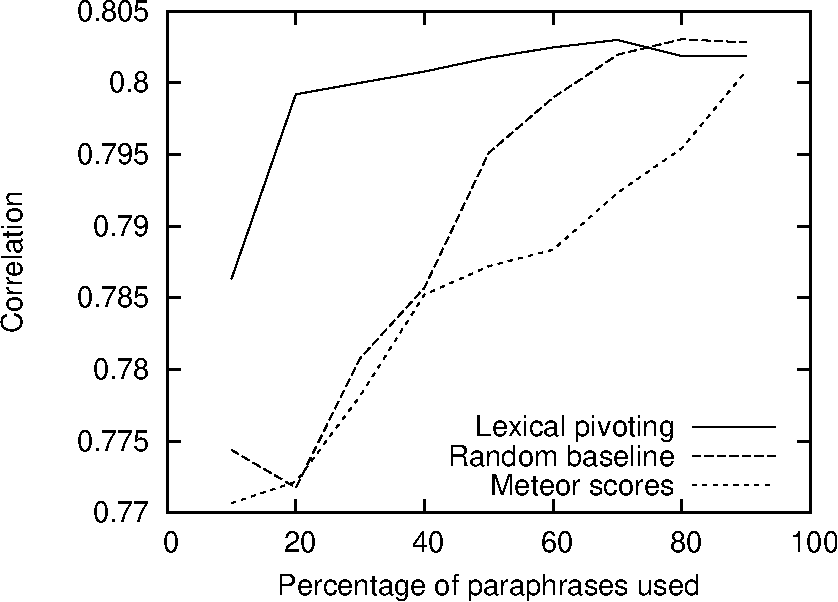
\includegraphics[scale=0.80]{../img/filtering-lexical-cropped.pdf}
\caption{Correlation between human judgments and \bleu scores computed on paraphrased references produced by the ~\emph{One-word only} strategy, using the top $0, 10, 20,\ldots,90\% $ paraphrases from \fm selected by automatic filtering techniques: random baseline, \meteor score, and lexical pivoting on WMT12 data.}
\label{fig:filtering-lexical}
\end{figure}

\begin{figure}[tb!]
\centering
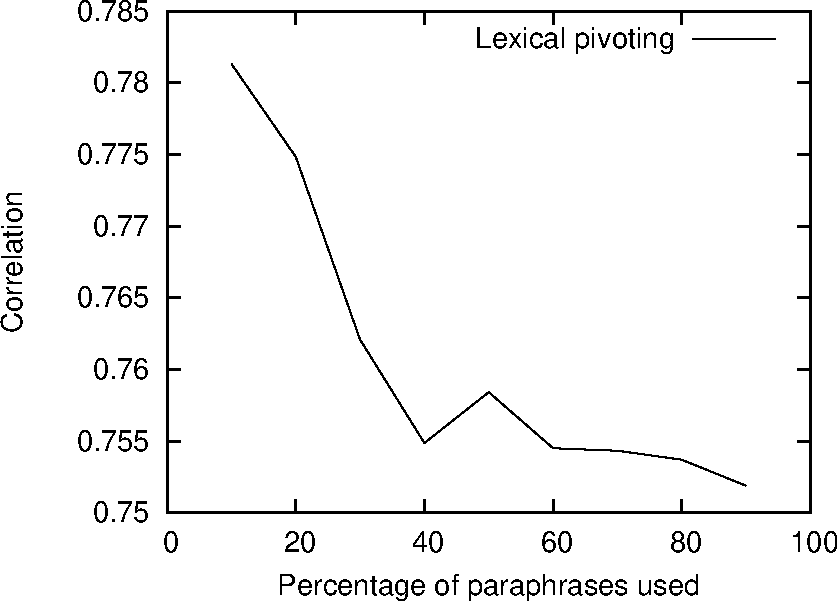
\includegraphics[scale=0.8]{../img/filtering-mwe-cropped.pdf}
\caption{Correlation between human judgments and \bleu scores computed on paraphrased references produced by the ~\emph{Multi-word-first} strategy, using the top $0, 10, 20,\ldots,90\% $ paraphrases from \cmpt selected by lexical pivoting on WMT12 data.}
\label{fig:filtering-mwe}
\end{figure}

We further evaluate the best-performing technique---lexical pivoting---by applying it to filter multi-word paraphrases from \cmpt. \Cref{fig:filtering-mwe} shows considerable improvement in correlation with a decreasing number of used paraphrases. Lexical pivoting successfully mitigated the impact from noisy entries, with correlation increasing as the table is pruned. However, even at the peak performance (using only the top 10\% of paraphrases), the results did not outperform the \emph{One-word only} strategy. 

Consequently, while automatic filtering—specifically lexical pivoting—is an effective approach to noise reduction, it does not provide a meaningful improvement over the heuristic-based \fm tables. For this reason, we utilize the unfiltered \fm and \wordnet for our primary experiments.

\section*{Example of distributional similarity computation}
\label{app:distributional}
\addcontentsline{toc}{section}{Example of distributional similarity computation} 

To illustrate the computation of cosine similarity in the context of text analysis, we use a simple corpus to demonstrate how this measurement can be calculated to assess the similarity between word distributions. The process begins with constructing a co-occurrence matrix within sentences
from a given corpus. Consider a corpus consisting of the following three sentences:

\begin{enumerate}
    \item Birds fly high, birds fly fast.
    \item Fly high, fly often.
    \item Often birds sing loudly.
\end{enumerate}

In the first step, we split sentences into words, remove punctuation, and lowercase all words. In this example, we focus on the window size of 1, which means that we are only considering immediate neighbors within a sentence. In this co-occurrence matrix  (\Tref{table:distribution-semantics}), word order is not taken into account, resulting in a symmetrical structure. Each entry in the matrix represents the frequency with which each word appears adjacent to another, regardless of whether it appears before or after. 

\begin{table}[h]
\centering
\begin{tabular}{|c|ccccccc|}
\hline
\textbf{Word} & \textbf{birds} & \textbf{fast} & \textbf{fly} & \textbf{high} & \textbf{loudly} & \textbf{often} & \textbf{sing} \\
\hline
birds  & [0, & 0, & 2, & 1, & 0, & 1, & 1] \\
fast   & [0, & 0, & 1, & 0, & 0, & 0, & 0] \\
fly    & [2, & 1, & 0, & 3, & 0, & 1, & 0] \\
high   & [1, & 0, & 3, & 0, & 0, & 0, & 0] \\
loudly & [0, & 0, & 0, & 0, & 0, & 0, & 1] \\
often  & [1, & 0, & 1, & 0, & 0, & 0, & 0] \\
sing   & [1, & 0, & 0, & 0, & 1, & 0, & 0] \\
\hline
\end{tabular}

\caption{The co-occurrence matrix presented here is computed from the simple three-sentence corpus, using the context window size of 1 and ignoring word order. This matrix illustrates how frequently each word appears adjacent to every other word within the corpus.}

%We calculate the cosine similarity between these to quantify the similarity of their distribution.
%In this example, the cosine similarity is approximately 0.35 suggesting relatively small degree of similarity
%between the contexts of paraphrase pairs \textit{Often} and \textit{Loudly}.}
\label{table:distribution-semantics}
\end{table}

From the matrix, we can derive context vectors for the words "fly" and "sing" based on their immediate neighbors:

Context(fly) = [2, 1, 0, 3, 0, 1, 0]

Context(sing) = [1, 0, 0, 0, 1, 0, 0] 

We calculate the cosine similarity between these two vectors to quantify the similarity of their distribution. 

\begin{equation}
\nonumber
  \begin{aligned}
    \text{CS(fly,sing)} & = \frac{Context(fly) \cdot Context(sing)} {\|Context(fly)\| \|Context(sing)\|} \\
                     & = \frac{(2 \times 1) + (1 \times 0) + ... % (0 \times 0) + (3 \times 0) + (0 \times 1) 
                     + (1 \times 0) + (0 \times 0) }{\sqrt{2^2 + 1^2 + 0^2 + 3^2 + 0^2 
                     + 1^2 + 0^2} \sqrt{1^2 + 0^2 + 0^2 + 0^2 + 1^2 + ...}} \\
              %       + 1^2 + 0^2} \sqrt{1^2 + 0^2 + 0^2 + 0^2 + 1^2 + 0^2 + 0^2}}\\
                     & =  \frac{2}{\sqrt{15}\sqrt{2}} \\
                     & \approx 0.37 
  \end{aligned}
\end{equation}


In this example, the cosine similarity is approximately 0.37 suggesting a relatively small degree of similarity between the contexts of word \textit{fly} and \textit{sing}. 